\section{Literature Review}

\subsection{Motor-sport Aerodynamics}
In 1949 Ludwig Prandtl stated, "The term aerodynamics is generally used for problem arising from flight and other topics involving the flow of air\cite{Anderson2007FundamentalsJr.}". By definition, Aerodynamics is one of the branch in physics which concern and study the interaction of a body and fluid flow stream\cite{Scibor-Rylski1984RoadAerodynamics}. The forces' magnitude and direction occur on a body is a result of the flow interaction which depends on several variables. Some fundamental variables in aerodynamics include flow velocity, temperature, pressure, and density, which further describe the flow physics and characteristic. Drag and lift are the greatest consideration in race-car aerodynamic which will be discussed further on next subsection on this paper.

Aerodynamics is generally classified into external (flow around  the body) and internal (flow inside the body). This paper will focus on external aerodynamics which focus on the force generation due to the air-stream behaviour around the body of interest. In the automotive industry, external force plays an important part since the overall performance of the car is dependent on the aerodynamics forces created which significantly influence and improve the vehicle shape to its aerodynamics advantage \cite{Scibor-Rylski1984RoadAerodynamics}. Some of the aerodynamics consideration to vehicle's shape influence include large downforce generation, downforce balance between from and rear tyre, and drag minimisation. Table\ref{Table1} shows the effect of downforce to a racing car's acceleration, it can be seen that downforce significantly improve the acceleration time by -1.06 seconds, rate of acceleration by 4.5 $m/s^2$, and power by 124 kilowatt. 

\begin{table}[!ht]
\caption{\label{Table1} Aerodynamic downforce effect of a racing car acceleration\cite{Scibor-Rylski1984RoadAerodynamics}.}
\begin{center}
 \begin{tabular}{||c| c c ||} 
 \hline
 Variables & With Downforce & Without Downforce \\ [0.5ex] 
 \hline\hline
 Time from 0 to 160 $km/h$ & 5s & 6.06s \\ 
 \hline
 Rate of acceleration at 44 $m/s$ & 10.02 $m/s^{2}$ & 5.52 $m/s^2$ \\
 \hline
 Power transferred at 44 $m/s^2$ & 353 kW & 229 kW  \\
 \hline

\end{tabular}
\end{center}
\end{table}

Queen's Formula Racing has started to focus on aerodynamics since 2016. Previous students have attempted to analyse the previous QFR car including undertray to optimise its overall performance.  This paper will solely focus on external aerodynamics to understand the flow behaviour of a QFR undertray and its force generation, which then the analyses are used for geometry consideration of the aerodynamic undertray.

\subsection{Aerodynamics Fundamental}
To fully understand the flow physics and behaviour of the aerodynamic undertray, there are several fundamental understanding or terminologies of aerodynamics which needs to be firstly understood.

\subsubsection{Flow Types}
The main characteristic of a liquid is the molecule ability to freely move around the space. The movement of liquid molecule to another point in space also requires energy, mass, and momentum to be transferred with it. In this occasion the "transfer phenomena" occurred, where the molecules introduced to viscosity (friction), thermal conduction, and mass diffusion \cite{Anderson2007FundamentalsJr.}. The flow that shows the indication of "transfer phenomena" can be called as viscous flow. On the other hand, the flow condition where the "transfer phenomena" does not occur is known as inviscid flow.

\noindent Some flow such as streamline far from wall can be represented by the inviscid flow. But to capture the aerodynamic behaviour between two near moving wall such an undertray, the viscous flow plays a crucial factor. The shear stress near wall boundaries is occurred by the presence of viscosity which become one of the major source in drag, as well the presence of viscosity allows us to capture flow separation on the high incident geometries. Viscous effect is important consideration in the analysis where the body of interest is purposely designed to generate aerodynamic forces due to the flow such as, airfoil and undertray.

\noindent Another important properties in aerodynamics is density ($\rho$). Compressibility on a flow is fully dependant on the the state of its density at certain speed. Incompressible flow can be referred to a flow with constant density throughout, which usually happen at the region of Mach number less than 0.3. In contrast the region of Mach greater than 0.3 is known as compressible flow where density is variable\cite{Anderson2007FundamentalsJr.}.

\subsubsection{Reynolds Number}
%talk about reybold Number as well how it affects the flow characteristic
Reynolds number is a dimensionless ratio of inertial and viscous forces which used to classify the probability of flow being laminar or turbulent\cite{Rehm2008SituationalMPD}. Mathematically, Reynolds Number can be expressed as:

\begin{equation}
Re = \frac{\rho v d}{\mu} = \frac{inertial force}{viscous force}
\end{equation}

\noindent For low Reynolds number, the flow can be categorised as laminar where the molecules move in a regular, smooth, steady, and no mixing between layer occurred\cite{Obidi2014TheoryVehicles}. In contrast the turbulent flow usually occur at high Reynolds number where the fluid particles travel in random and irregular attitude in which break up the streamline. When the flow is changing from laminar to turbulent, this flow is called transition region. Figure \ref{fig:2} shows the difference in laminar flow with transition to turbulent region near the wall. 

\begin{figure}[!ht]
    \centering
    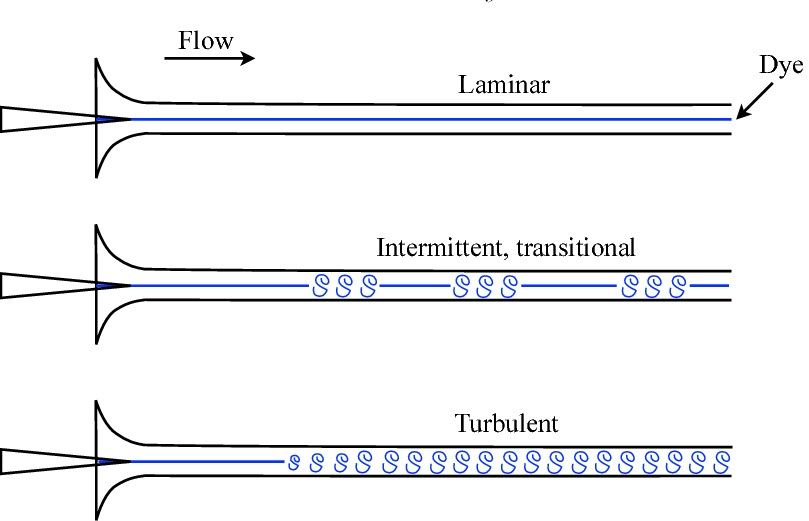
\includegraphics[scale=0.4]{Figures/laminar_turbulent_difference.jpg}
    \caption{Illustration of difference between laminar, transition, and turbulent flow in a pipe \cite{D.BARKLE2016TheoreticalPipe}.}
    \label{fig:2}
\end{figure}

\subsubsection{Boundary Layer}


\subsubsection{Bernoulli Equation}



\subsubsection{Aerodynamic Forces}
%due to to flow around the body there are some generation of force occured etc
Lift

Drag



\subsection{Aerodynamic Undertray}
% talk about what is it in general, how it improves and how it works etc and there are some governing understading behind this phenomena
\subsubsection{Ground Effect}
\subsubsection{Venturi Effect}
\subsubsection{Undertray devices}
